%%%%%%%%%%%%%%%%%%%%%%%%%%%%%%%%%%
% EL/EEE D1 Report Template
% University of Southampton
%
% author : Rhys Thomas (rt8g15)
%
% edited : 2016-11-14
%%%%%%%%%%%%%%%%%%%%%%%%%%%%%%%%%%

\documentclass[a4paper,11pt]{article}

%%%%%%%%%%%%%%%%%%%%%%%%%%%%%%%%%%
% PACKAGES
%%%%%%%%%%%%%%%%%%%%%%%%%%%%%%%%%%
\usepackage[margin=1in]{geometry}
\renewcommand{\baselinestretch}{1.2} % line spacing
\usepackage{color}
\usepackage{siunitx}
\usepackage{graphicx}
\usepackage{epstopdf}
\usepackage{float}
\usepackage{hyperref}
\usepackage{mathtools}
\usepackage[titletoc,toc,title]{appendix}
\usepackage{subfiles}
\usepackage{pgfplots}
\usepackage[european]{circuitikz}
\usepackage{textgreek}
\usepackage{amssymb}
\usepackage{subfig}

\pgfplotsset{compat=1.13}
\pgfplotsset{unit code/.code={\si{#1}}}
\usepgfplotslibrary{units}

\graphicspath{ {./images/} }

\usepackage{newunicodechar}
\newunicodechar{p}{\ifmmode\pi\else\textpi\fi}

%%%%%%%%%%%%%%%%%%%%%%%%%%%%%%%%%%
% DOCUMENT BEGIN
%%%%%%%%%%%%%%%%%%%%%%%%%%%%%%%%%%
\begin{document}
  
\begin{center}
{\Large{\textbf{ELEC2205 D3 -- Two-Stage Amplifier Design}}} \\ [\baselineskip]
\subfile{info.tex}
\end{center}

\begin{abstract}
\end{abstract}

\tableofcontents
\newpage

\section{Theoretical Design}
    The amplifier designed was a two-stage amplifier, consisting of a common emitter stage, and a common collector stage, in that order. Ideally, an amlifier should have a very high input impedance in order to avoid loading the source, and a very low output impedance. A common emitter provides a high input impedance, and a common collector provides a low output impedance, hence the order.
    
    \subsection{Derivations}
        \subsubsection{Stage 1 - Voltage Gain}

            \begin{figure}[h]
            \centering
                \subfile{./circuits/stage1Circuit.tex}
                \caption{Circuit diagram of the first stage of the amplifier. This is the common emitter stage.}
                \label{fig:stage1}
            \end{figure}

            In order to derive the voltage gain of this circuit, we need to analyse it using a small signal model. The hybrid-\textpi\ model (figure~\ref{fig:stage1hpi}) will be used.

            \begin{figure}[h]
            \centering
                \subfile{./circuits/stage1hpi.tex}
                \caption{Hybrid-\textpi\ model of the first stage of the amplifier.}
                \label{fig:stage1hpi}
            \end{figure}

            Using Kirchoff's current law on the base:

            \begin{subequations}
            \begin{align}
                \frac{v_b - v_s}{R_s} + \frac{v_b}{R_2} + \frac{v_b}{R_1} + \frac{v_b - v_e}{r_\pi} &= 0\\
                \frac{v_b - v_s}{R_s} + v_b \left(\frac{1}{R_1} + \frac{1}{R_2} \right) + \frac{v_b - v_e}{r_\pi} &= 0 \label{eq:kclBase}
            \end{align}
            \end{subequations}

            It can be seen that $v_\pi = v_b - v_e$. The small signal output resistance, $r_\pi$, is defined as $\frac{\beta}{g_m}$~\cite[p. 29]{ADAIC}.

            Using Kirchoff's current law on the emitter:

            \begin{subequations}
            \begin{align}
                &\frac{v_e - v_b}{r_\pi} - g_m (v_b - v_e) + \frac{v_e}{R_{e2}} + \frac{v_e - v_c}{r_0} = 0\\
                \textrm{Assuming $r_0$ is large: } &\frac{v_e - v_b}{r_\pi} - g_m (v_b - v_e) + \frac{v_e}{R_{e2}} = 0 \label{eq:kclEmitter}
            \end{align}
            \end{subequations}

            Using Kirchoff's current law on the collector:

            \begin{equation} \label{eq:kclCollector}
                \frac{v_c}{R_c} + g_m(v_b - v_e) = 0
            \end{equation}

            After some tedious manipulation
            
            \begin{equation} \label{eq:s1gain}
                \frac{v_c}{v_b} = \frac{-g_m R_c}{1 + g_m R_e \left( 1+ \frac{1}{\beta} \right) }
                                = \frac{-\beta R_c}{r_{\pi} + R_e (\beta + 1)}
            \end{equation}
            
            \subsubsection{Stage 1 - Impedance}
                
            We can also work out the impedance of the base terminal
            
            \begin{subequations}
            \begin{align}
                R_b &= \frac{v_b}{i_b}\\
                    &= \frac{v_b}{(v_b - v_e) / r_{\pi}}\\
                    &= \frac{r_{\pi}}{1 - (v_e / v_b)}\\
                    &= r_{\pi} \left( 1 + g_m R_e \left( 1 + \frac{1}{\beta} \right) \right)\\
                    &= r_{\pi} + R_e (\beta + 1)
            \end{align}
            \end{subequations}
            
            Looking at the hybrid-\textpi model (figure \ref{fig:stage1hpi}), we can see that the overall impedance is therefore the parallel combination of $R_2$, $R_1$, and $R_b$.
            
            \begin{equation}
                R_{in} = \left( \frac{1}{R_1} + \frac{1}{R_2} + \frac{1}{r_{\pi} + R_e (\beta + 1)} \right) ^{-1}
            \end{equation}
            
        \newpage
        \subsubsection{Stage 2 - Voltage Gain}
            \begin{figure}[h]
            \centering
                \subfile{./circuits/stage2Circuit.tex}
                \caption{Circuit diagram of the second stage of the amplifier. This is the common collector stage.}
                \label{fig:stage2}
            \end{figure}
            
            \begin{figure}[h]
            \centering
                \subfile{./circuits/stage2hpi.tex}
                \caption{Hybrid-\textpi model of the second stage.}
                \label{fig:stage2hpi}
            \end{figure}
            
            Using Kirchoff's current law on the emitter
            
            \begin{equation}
                (\beta + 1) \frac{v_{in} - v_{out}}{R_s + \left( r_{\pi}^{-1} + R_{3}^{-1} + R_{4}^{-1} \right)^{-1}} = v_{out} \left( \frac{1}{R_L} + \frac{1}{r_o} \right)
            \end{equation}
            
            We can define some resistance values
            
            \begin{subequations} \label{eq:stage2res}
            \begin{gather}
                \frac{1}{R_E} = \frac{1}{R_L} + \frac{1}{r_o} \\
                R = \frac{R_s + \left( r_{\pi}^{-1} + R_{3}^{-1} + R_{4}^{-1} \right)^{-1}}{\beta + 1}
            \end{gather}
            \end{subequations}
            
            After some manipulation, the voltage gain can be written as
            
            \begin{equation} \label{eq:stage2gain}
                A_v = \frac{1}{1 + \frac{R}{R_E}}
            \end{equation}
            
        \subsubsection{Stage 2 - Impedance}
        
            The input impedance can be calculated like so~\cite{wikiCC}
            
            \begin{subequations}
            \begin{align}
                R_{in} &= \frac{v_{in}}{i_b} \\
                       &= \frac{R_s + \left( r_{\pi}^{-1} + R_{3}^{-1} + R_{4}^{-1} \right)^{-1}}{1 - A_v} \\
                       &= \left( R_s + \left( r_{\pi}^{-1} + R_{3}^{-1} + R_{4}^{-1} \right)^{-1} \right) \left( 1 + \frac{R_E}{R} \right) \\
                       &= R_s + \left( r_{\pi}^{-1} + R_{3}^{-1} + R_{4}^{-1} \right)^{-1} + R_E (\beta + 1)
            \end{align}
            \end{subequations}
            
            To calculate the output impedance, a current source, $i_\mathrm{x}$ is added, as shown in figure~\ref{fig:stage2hpi2}.
            
            \begin{figure}[h]
            \centering
                \subfile{./circuits/stage2hpi2.tex}
                \caption{Hybrid-\textpi model of the second stage for finding output impedance.}
                \label{fig:stage2hpi2}
            \end{figure}
            
            \begin{subequations}
            \begin{gather}
                R_{out} = \frac{v_\mathrm{x}}{i_\mathrm{x}} \\
                i_b (\beta + 1) = i_\mathrm{x} - \frac{v_\mathrm{x}}{R_E} \\
                v_\mathrm{x} = i_b (R_s + \left( r_{\pi}^{-1} + R_{3}^{-1} + R_{4}^{-1} \right)^{-1} ) \\
                R_{out} = \frac{v_\mathrm{x}}{i_\mathrm{x}} = \left( \frac{1}{R} + \frac{1}{R_E} \right)^{-1}
            \end{gather}
            \end{subequations}
            
    \subsection{Circuit Design}
        The resistor and capacitor values were found using an existing amplifier method: \cite{ampDesign}.

\newpage
\section{Voltage Gain Measurement}
    The voltage gain of each stage of the amplifier was measured by supplying an alternating voltage at the input, and measuring the amplitude of the voltage at the output. The gain of both stages combined was also measured this way. The measurements are shown in figure~\ref{fig:oscgain} and consolidated in table~\ref{tab:gain}.
    
    \begin{figure}[h]
        \centering
        \subfloat[Oscilloscope captures of input and output signals][Stage 1]
        {
            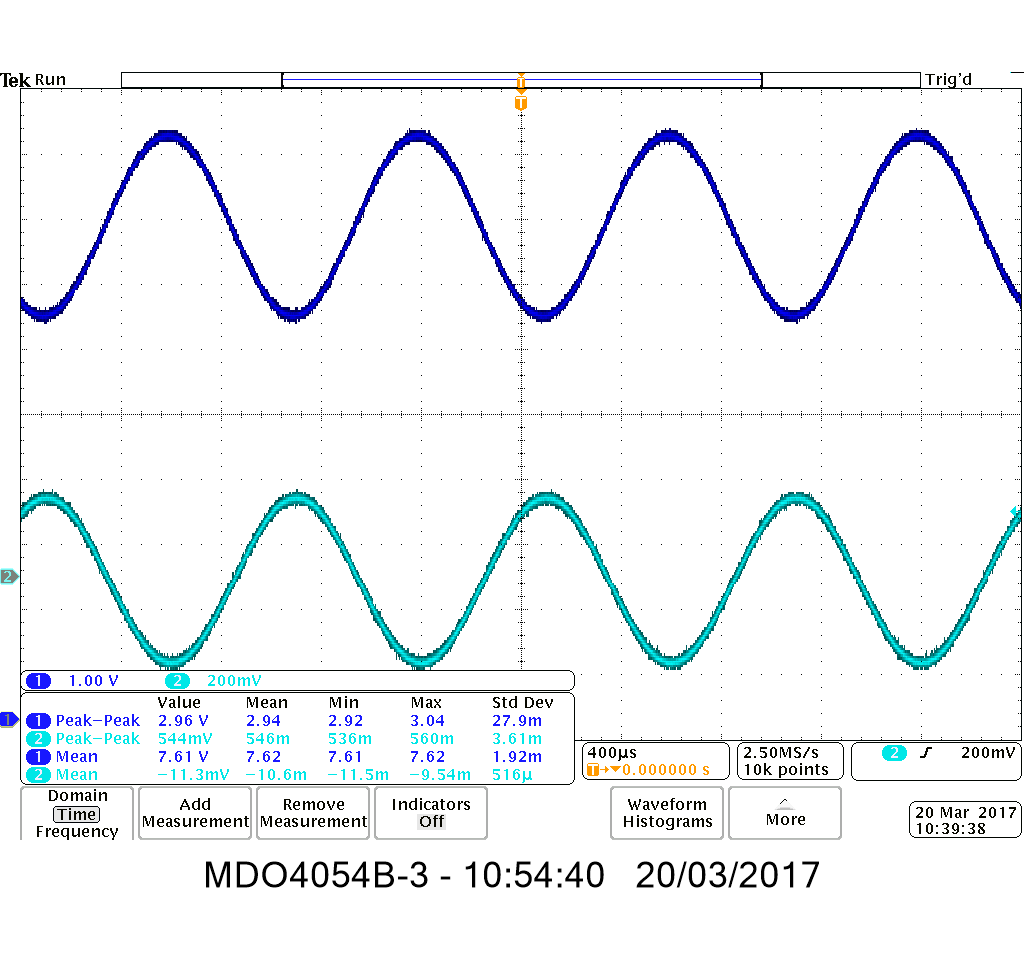
\includegraphics[width = 0.45\textwidth]{stage1gain.png}
            \label{fig:oscgain1}
        }
        \subfloat[Oscilloscope captures of input and output signals][Stage 2]
        {
            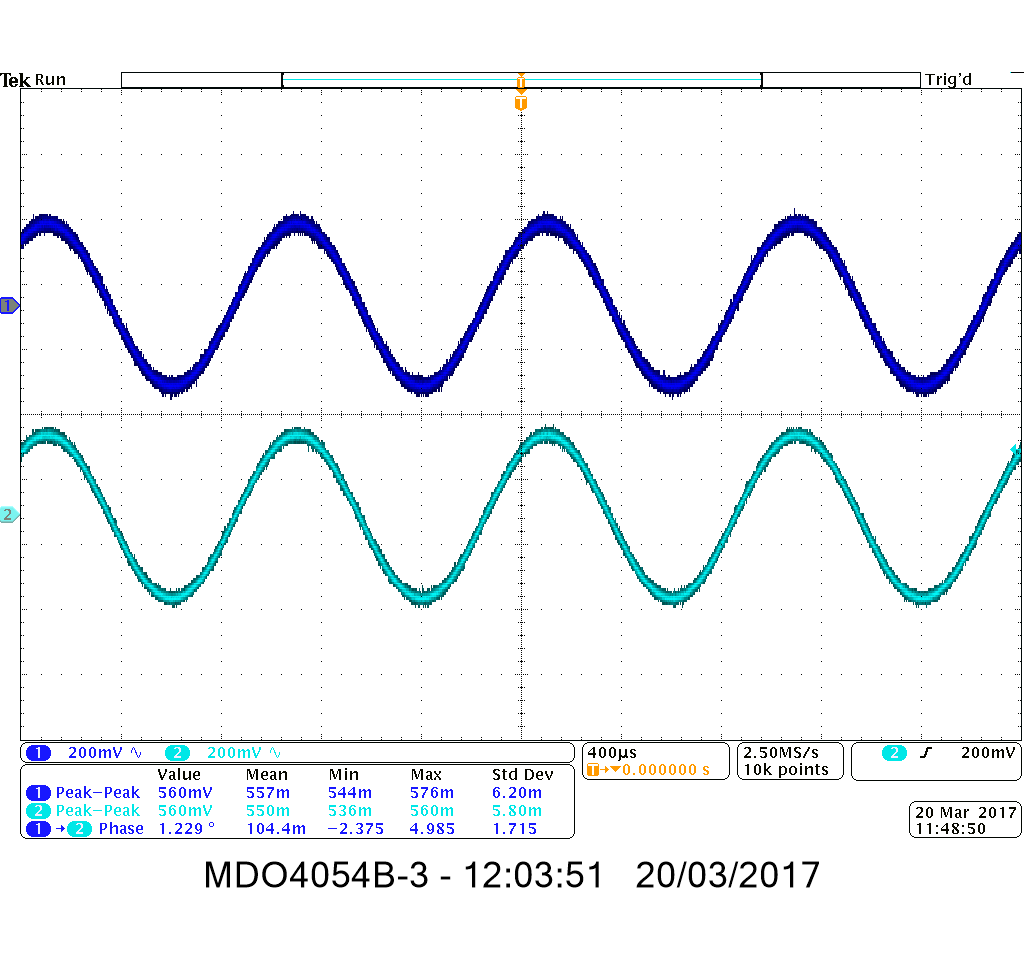
\includegraphics[width = 0.45\textwidth]{stage2gain.png}
            \label{fig:oscgain2}
        }
        \qquad
        \subfloat[Oscilloscope captures of input and output signals][Combined]
        {
            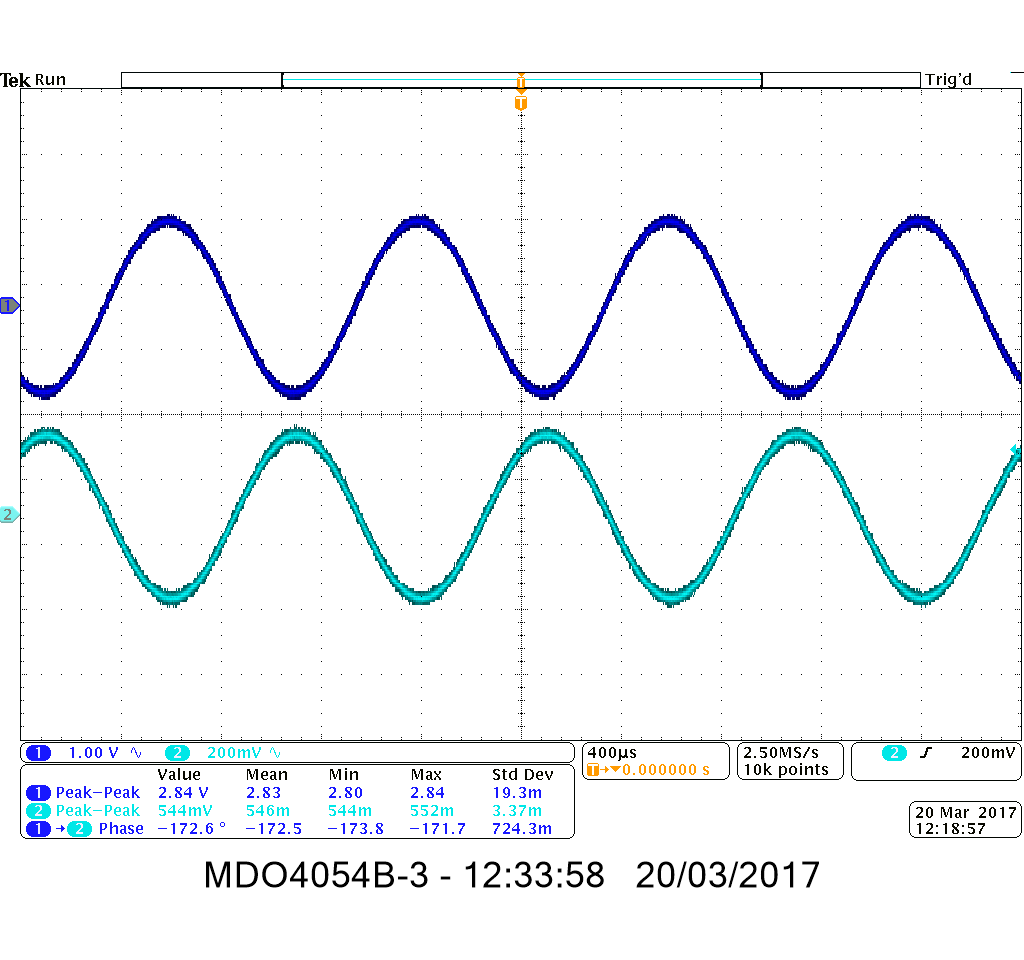
\includegraphics[width = 0.4\textwidth]{totalgain.png}
            \label{fig:oscgaintot}
        }
        \caption{Oscilloscope captures of input and output signals. The top waveform (2) in each image is the output, and the bottom (1) is the output.}
        \label{fig:oscgain}
    \end{figure}

    \begin{table}[h]
        \centering
        \subfloat[][Stage 1]
        {
            \begin{tabular}{|l|l|}
                \hline
                \textbf{Frequency}      & \SI{1}{\kilo\hertz}           \\ \hline
                \textbf{Input Voltage}  & \SI{500}{\milli\volt_{pp}}    \\ \hline
                \textbf{Output Voltage} & \SI{2.96}{\volt_{pp}}         \\ \hline
                \textbf{Gain}           & 5.92                          \\ \hline
            \end{tabular}
            \label{tab:s1gain}
        }
        \subfloat[][Stage 2]
        {
            \begin{tabular}{|l|l|}
                \hline
                \textbf{Frequency}      & \SI{1}{\kilo\hertz}           \\ \hline
                \textbf{Input Voltage}  & \SI{500}{\milli\volt_{pp}}    \\ \hline
                \textbf{Output Voltage} & \SI{558}{\milli\volt_{pp}}    \\ \hline
                \textbf{Gain}           & 1.01                          \\ \hline
            \end{tabular}
            \label{tab:s2gain}
        }
        \qquad
        \subfloat[][Combined]
        {
            \begin{tabular}{|l|l|}
                \hline
                \textbf{Frequency}      & \SI{1}{\kilo\hertz}           \\ \hline
                \textbf{Input Voltage}  & \SI{500}{\milli\volt_{pp}}    \\ \hline
                \textbf{Output Voltage} & \SI{2.83}{\volt_{pp}}         \\ \hline
                \textbf{Gain}           & 5.66                          \\ \hline
            \end{tabular}
            \label{tab:scombgain}
        }
        \subfloat[][Stage 1 with $C_e$ removed]
        {
            \begin{tabular}{|l|l|}
                \hline
                \textbf{Frequency}      & \SI{1}{\kilo\hertz}           \\ \hline
                \textbf{Input Voltage}  & \SI{500}{\milli\volt_{pp}}    \\ \hline
                \textbf{Output Voltage} & \SI{2.48}{\volt_{pp}}         \\ \hline
                \textbf{Gain}           & 4.96                          \\ \hline
            \end{tabular}
            \label{tab:scombgain}
        }
        \qquad
        \subfloat[][Stage 1 with $R_{e1}$ and $R_{e2}$ bridged]
        {
            \begin{tabular}{|l|l|}
                \hline
                \textbf{Frequency}      & \SI{1}{\kilo\hertz}           \\ \hline
                \textbf{Input Voltage}  & \SI{20}{\milli\volt_{pp}}    \\ \hline
                \textbf{Output Voltage} & \SI{1.413}{\volt_{pp}}         \\ \hline
                \textbf{Gain}           & 70.65                          \\ \hline
            \end{tabular}
            \label{tab:scombgain}
        }
        \caption{Tables of measurements made from the two amplifier stages, the amplifier with both stages combined, and for the advanced tasks.}
        \label{tab:gain}
    \end{table}
        
    \subsection{Frequency Response}
        The frequency and phase response of the combined amplifier was measured, and is shown in figure~\ref{fig:freqResponse}.
        
        \begin{figure}[h]
        \centering
            \subfloat[Frequency][Frequency response]{
                \begin{tikzpicture}
                    \begin{axis}[
                        width = \textwidth,
                        height = 0.3\textheight,
                        xlabel = {Frequency},
                        x unit = \si{\hertz},
                        ylabel = {Gain},
                        grid = both,
                        xmode = log
                        ]
                        \addplot table[x = Frequency, y = Gain, col sep = comma]{./tables/freqResponse.csv};
                    \end{axis}
                \end{tikzpicture}
                \label{plot:phase}
            }
            \qquad
            \subfloat[Phase][Phase response]{
                \begin{tikzpicture}
                    \begin{axis}[
                        width = \textwidth,
                        height = 0.3\textheight,
                        xlabel = {Frequency},
                        x unit = \si{\hertz},
                        ylabel = {Phase},
                        y unit = \si{\degree},
                        grid = both,
                        xmode = log
                        ]
                        \addplot table[x = Frequency, y = Phase2, col sep = comma]{./tables/freqResponse.csv};
                    \end{axis}
                \end{tikzpicture}
                \label{plot:frequency}
            }
            \caption{Bode plot of the combined two-stage amplifier.}
            \label{fig:freqResponse}
        \end{figure}

\newpage
\section{Impedance Measurement}
    Impedance values were calculated by measuring the voltage across a resistor with a value estimated to be near the actual impedance.
    
    \subsection{Stage 1}
        \subsubsection{Input impedance}
            \begin{figure}[h]
            \centering
                \subfile{./circuits/stage1InputImpedance.tex}
                \caption{Measuring the input impedance of the first amplification stage.}
                \label{fig:stage1inputZ}
            \end{figure}
            
            \begin{subequations} \label{eq:stage1Rin}
            \begin{align}
                \frac{V_{i1}}{V_{i1}'} &= \frac{R_{in1}}{R_{in1} + 47000}   \\
                \frac{79.2}{177} &= \frac{R_{in1}}{R_{in1} + 47000}   \\
                \therefore R_{in1} &= \SI{45.1}{\kilo\ohm}
            \end{align}
            \end{subequations}
            
            As shown by equation set~\ref{eq:stage1Rin}, the input impedance of stage 1 was calulated to be \SI{45.1}{\kilo\ohm}.
        
        \subsubsection{Output impedance}
        
            \begin{figure}[h]
            \centering
                \subfile{./circuits/stage1OutputImpedance.tex}
                \caption{Measuring the output impedance of the first amplification stage.}
                \label{fig:stage1outputZ}
            \end{figure}
            
            \begin{subequations} \label{eq:stage1Rout}
            \begin{align}
                \frac{V_{o1}}{V_{o1}'} &= \frac{R_{out1}}{R_{out1} + 47000}   \\
                \frac{265}{530} &= \frac{R_{out1}}{R_{out1} + 47000}   \\
                \therefore R_{out1} &= \SI{1.8}{\kilo\ohm}
            \end{align}
            \end{subequations}
            
            As shown by equation set~\ref{eq:stage1Rout}, the output impedance of stage 1 was calulated to be \SI{1.8}{\kilo\ohm}.
        
    \subsection{Stage 2}
        \subsubsection{Input impedance}
            \begin{figure}[h]
            \centering
                \subfile{./circuits/stage2InputImpedance.tex}
                \caption{Measuring the input impedance of the second amplification stage.}
                \label{fig:stage2inputZ}
            \end{figure}
            
            \begin{subequations} \label{eq:stage2Rin}
            \begin{align}
                \frac{V_{i2}}{V_{i2}'} &= \frac{R_{in2}}{R_{in2} + 27000}   \\
                \frac{111}{177} &= \frac{R_{in2}}{R_{in2} + 27000}   \\
                \therefore R_{in2} &= \SI{45.4}{\kilo\ohm}
            \end{align}
            \end{subequations}
            
            As shown by equation set~\ref{eq:stage2Rin}, the input impedance of stage 2 was calulated to be \SI{45.4}{\kilo\ohm}.
    
        \subsubsection{Output impedance}
            \begin{figure}[h]
            \centering
                \subfile{./circuits/stage2OutputImpedance.tex}
                \caption{Measuring the output impedance of the second amplification stage.}
                \label{fig:stage2outputZ}
            \end{figure}
            
            \begin{subequations} \label{eq:stage2Rout}
            \begin{align}
                \frac{V_{o2}}{V_{o2}'} &= \frac{R_{out2}}{R_{out2} + 68}   \\
                \frac{66}{178} &= \frac{R_{out2}}{R_{out2} + 68}   \\
                \therefore R_{out2} &= \SI{40.1}{\ohm}
            \end{align}
            \end{subequations}
            
            As shown by equation set~\ref{eq:stage2Rout}, the output impedance of stage 2 was calulated to be \SI{40.1}{\ohm}.
            
    \subsection{Combined}
        \subsubsection{Input impedance}
            This was measured using the same method as when measuring the input impedance of the first stage alone.
            
            \begin{subequations} \label{eq:Rin}
            \begin{align}
                \frac{V_{i}}{V_{i}'} &= \frac{R_{in}}{R_{in} + 47000}   \\
                \frac{86.2}{177} &= \frac{R_{in}}{R_{in} + 47000}   \\
                \therefore R_{in} &= \SI{44.6}{\kilo\ohm}
            \end{align}
            \end{subequations}
            
            As shown by equation set~\ref{eq:Rin}, the input impedance of the combined amplifier was calulated to be \SI{44.6}{\kilo\ohm}.
            
        \subsubsection{Output impedance}
            This was measured using the same method as when measuring the output impedance of the second stage alone.
            
            \begin{subequations} \label{eq:Rout}
            \begin{align}
                \frac{V_{o}}{V_{o}'} &= \frac{R_{in}}{R_{out} + 68}   \\
                \frac{147}{929} &= \frac{R_{out}}{R_{out} + 68}   \\
                \therefore R_{out} &= \SI{12.8}{\ohm}
            \end{align}
            \end{subequations}
            
            As shown by equation set~\ref{eq:Rout}, the output impedance of the combined amplifier was calulated to be \SI{12.8}{\ohm}.

\newpage
\section{Reflection or w/e}

\newpage
\begin{appendices}
    \label{appendix}
    \section{Some appendix}
    \label{app:one}
\end{appendices}

\bibliographystyle{IEEEtran}
% IEEEabrv abbreviates journal titles in accordance to IEEE standards 
\bibliography{mybib}

\end{document}